% ============================================================
% Uncertainty Propagation in Tree-Structured Language Model Reasoning
% Daniel Ray Edgar
% ============================================================
\documentclass[11pt]{article}

\usepackage[margin=1.25in]{geometry}
\usepackage{natbib}
\usepackage{amsmath,amssymb,amsthm}
\usepackage{mathtools}
\usepackage{dsfont}
\usepackage{bm}
\usepackage{graphicx}
\usepackage{xcolor}
\usepackage{hyperref}
\usepackage{booktabs}
\usepackage{array}
\usepackage{multirow}
\usepackage{caption}
\usepackage{subcaption}
\usepackage{enumitem}
\usepackage{nicefrac}
\usepackage{microtype}
\usepackage{tikz}
\usepackage{pgfplots}
\usepackage{pgfplotstable}
\usepackage{algorithm}
\usepackage{algpseudocode}
\pgfplotsset{compat=1.18}
\usepgfplotslibrary{colormaps}
\usetikzlibrary{arrows.meta, positioning, shapes.geometric, fit, calc, backgrounds}

\definecolor{darkblue}{RGB}{0,60,120}
\definecolor{medblue}{RGB}{0,100,200}
\definecolor{lightblue}{RGB}{173,216,255}
\definecolor{darkgray}{RGB}{80,80,80}
\definecolor{medgray}{RGB}{150,150,150}

\hypersetup{colorlinks=true, linkcolor=darkblue, citecolor=darkblue, urlcolor=medblue}

\theoremstyle{plain}
\newtheorem{theorem}{Theorem}[section]
\newtheorem{lemma}[theorem]{Lemma}
\newtheorem{proposition}[theorem]{Proposition}
\newtheorem{corollary}[theorem]{Corollary}

\theoremstyle{definition}
\newtheorem{definition}[theorem]{Definition}
\newtheorem{example}[theorem]{Example}
\newtheorem{remark}[theorem]{Remark}
\newtheorem{assumption}[theorem]{Assumption}

\newcommand{\E}{\mathbb{E}}
\newcommand{\Var}{\mathrm{Var}}
\newcommand{\Cov}{\mathrm{Cov}}
\newcommand{\Prob}{\mathbb{P}}
\newcommand{\R}{\mathbb{R}}
\newcommand{\N}{\mathbb{N}}
\newcommand{\llm}{\mathcal{M}}
\newcommand{\tree}{\mathcal{T}}
\newcommand{\chain}{\mathcal{C}}
\newcommand{\thetavec}{\bm{\theta}}
\newcommand{\correct}{\textsc{correct}}
\newcommand{\BigO}{\mathcal{O}}
\DeclareMathOperator*{\argmax}{arg\,max}
\DeclareMathOperator*{\argmin}{arg\,min}

\title{%
  \vspace{-0.5cm}
  \textbf{Uncertainty Propagation in Tree-Structured}\\[2pt]
  \textbf{Language Model Reasoning}
  \vspace{0.3cm}
}

\author{Daniel Ray Edgar}
\date{\normalsize\today}

% ============================================================
\begin{document}
\maketitle
\thispagestyle{empty}

\begin{abstract}
This paper asks a question I kept running into while working with modern language
models and could not find a satisfying answer to in the literature: when a model
executes a multi-step reasoning chain, how do small per-step mistakes accumulate
into end-to-end failure, and does the answer change if you branch the reasoning
into a tree instead of a line? I set up a simple probabilistic model (each
reasoning step is an independent Bernoulli trial with its own failure probability
$\theta_i$) and work out the math from there. For a depth-$n$ chain the answer
comes out to $\prod_{i=1}^n(1-\theta_i)$, which decays exponentially in $n$. For
a $k$-ary tree with majority vote I prove a Hoeffding bound that gives
sub-exponential decay. I also work out the maximum-likelihood estimators for the
$\theta_i$ from labeled trajectory data and obtain confidence intervals via the
delta method. To test whether any of this matches reality, I ran the framework
against GPT-5, Claude Opus 4.6, Claude Sonnet 4.6, and Gemini 3.1 Pro on
GSM8K, MATH, and MMLU-Pro. The fitted predictions track empirical success rates
to within $1\%$ mean absolute error across all four models, and switching from a
linear chain to a depth-3 branching tree at a fixed compute budget of 48 steps
raises success probability from roughly $18\%$ to $96\%$ on MATH-level problems.
The core finding is that the exponential decay is real and severe even for the
best models currently available, and that tree branching is not a marginal
improvement. It is a qualitatively different operating regime.
\end{abstract}

\newpage
\setcounter{page}{1}

% ============================================================
\section{Introduction}
\label{sec:intro}
% ============================================================

I got interested in this problem in an applied context, not a theoretical one.
I was building systems that used language models to do multi-step analysis, the
kind of work where the model has to set up a problem, do several intermediate
calculations, and produce a final answer, and I kept noticing that accuracy
degraded badly as tasks got longer, even when each individual step looked fine.
My first instinct was that it was a prompting issue. After a while I started
to wonder if the problem was more fundamental than that.

The calculation that changed how I thought about it is embarrassingly simple.
If a model has a $10\%$ chance of getting any single step wrong, and you ask it
to do ten steps, the probability of getting all ten right is $0.9^{10} \approx
35\%$. That is it. No fancy reasoning needed. What surprised me was how few
papers seemed to have actually said this out loud in a rigorous way. There is an
enormous literature on chain-of-thought prompting \citep{wei2022chain,
kojima2022large}, self-consistency \citep{wang2022self}, and tree-of-thought
search \citep{yao2023tree}, and all of it is implicitly about managing exactly
this problem, but the underlying probabilistic structure is almost never written
down explicitly. I wanted to write it down.

The setup I landed on is what I call the \textbf{Reasoning Tree Model (RTM)}.
Each step in a reasoning trace is modeled as a Bernoulli trial with a
step-specific failure probability $\theta_i$, and the steps are assumed
independent of each other given the query. Under these two assumptions, which
I think are reasonable approximations and I check empirically in
Section~\ref{sec:experiments}, the math becomes tractable enough to produce
genuinely useful closed forms.

For chains, the result is Theorem~\ref{thm:chain}: success probability is
exactly $\prod_{i=1}^n(1-\theta_i)$, and it decays exponentially. For trees
with majority vote, Theorem~\ref{thm:subexp} gives a Hoeffding-type bound
showing the decay is sub-exponential in total compute. I also characterize
where the optimum is (the right tree depth and branching factor for a given
error rate and step budget), and the answer (Theorem~\ref{thm:optk}) turns
out to be shallow trees with moderate branching, not the deep expansive search
that tree-of-thought papers sometimes imply.

On the estimation side, the MLE for the step parameters is just the empirical
error rate at each step (Theorem~\ref{thm:mle}), which is reassuringly
boring. The interesting piece is propagating the estimation uncertainty through
the product to get confidence intervals on end-to-end success probability, which
requires the delta method (Theorem~\ref{thm:ci}).

I want to be honest about what I don't do here. I don't model the internal
mechanics of how one wrong step influences the next. The step-wise independence
assumption is an idealization. I don't handle adaptive search strategies like
value-guided beam search, which are more common in practice than the uniform
tree expansion I analyze. And I have not derived any generalization bounds
across problem types. This is, as far as I can tell, a first pass at the
problem, not a final word on it.

\paragraph{Relation to prior work.}
The work that came closest to what I was trying to do when I started is
\citet{li2024cascade}, which models error cascades in tool-augmented agents. But
their model is built around Markov-dependent tool-call states, not branching
reasoning trees, and the estimation framework is different. The self-consistency
paper \citep{wang2022self} is the empirical precursor to the tree analysis in
Section~\ref{sec:trees}, where it is effectively depth-1 tree search, but it does
not characterize the optimal structure. Process reward models
\citep{lightman2023let} collect exactly the kind of step-level labels my
estimator needs, though they use those labels to train a dense reward signal
rather than to estimate failure parameters. More recent work on reliability in
agentic systems \citep{zhao2024reliability} touches adjacent territory but
focuses on tool failures rather than reasoning steps. The conformal and
entropy-based uncertainty methods \citep{angelopoulos2023conformal,
kuhn2023semantic} are useful for output-level certificates but don't model
the structural source of the uncertainty. As far as I can find, nobody has
written down the exact propagation formula for heterogeneous step errors across
tree topologies together with MLE theory. That is what this paper does.

% ============================================================
\section{The Reasoning Tree Model}
\label{sec:model}
% ============================================================

\subsection{Setup and Notation}

Let $\llm$ be a fixed language model. A reasoning problem is a pair $(q, a^*)$
where $q$ is the query and $a^*$ is the correct answer. Given $q$, the model
produces a trajectory $\tau = (s_1, \ldots, s_n, a)$ consisting of $n$
intermediate reasoning steps and a final answer.

\begin{definition}[Reasoning Step]\label{def:step}
  Step $s_i$ is the $i$-th token span generated by $\llm$ between designated
  delimiters (e.g., ``Step $i$:''\ \ldots\ ``Step $i{+}1$:''). It is
  \emph{correct} if its logical content constitutes a valid inference from
  $(q, s_1, \ldots, s_{i-1})$, and \emph{incorrect} otherwise.
\end{definition}

Write $X_i \in \{0,1\}$ for the correctness indicator of step $i$. I take the
final answer to be correct if and only if every step is correct.\footnote{This
is the standard assumption in the process reward model literature
\citep{lightman2023let}. Section~\ref{sec:model-extensions} discusses what
happens when you relax it.}

\begin{assumption}[Step-wise Independence]\label{ass:independence}
  Conditioned on $q$, the indicators $X_1,\ldots,X_n$ are mutually independent:
  \[
    \Prob(X_1=x_1,\ldots,X_n=x_n \mid q) = \prod_{i=1}^n \Prob(X_i=x_i \mid q).
  \]
\end{assumption}

\begin{assumption}[Bernoulli Steps]\label{ass:bernoulli}
  Each $X_i \sim \mathrm{Bernoulli}(1-\theta_i)$ for $\theta_i \in [0,1]$,
  the failure probability of step $i$. The vector
  $\thetavec = (\theta_1,\ldots,\theta_n) \in [0,1]^n$ is unknown.
\end{assumption}

Assumption~\ref{ass:independence} is the one I was most unsure about when
setting this up. The concern is that if a model enters a wrong ``mode'' early
in a chain, that error propagates forward and creates correlation between
subsequent step failures. In practice, as I measure in
Section~\ref{sec:experiments}, pairwise step correlations turn out to be
small (median $|\hat\rho_{ij}| < 0.04$ across the benchmarks I tested), so
the independence assumption seems like a reasonable working approximation.

\subsection{Chains and Trees}

\begin{definition}[Reasoning Chain]\label{def:chain}
  A reasoning chain $\chain_n$ is a directed path
  $s_1 \to s_2 \to \cdots \to s_n \to a$.
  It is correct iff all $n$ steps are correct.
\end{definition}

\begin{definition}[Reasoning Tree]\label{def:tree}
  A reasoning tree $\tree_{k,d}$ is a balanced $k$-ary tree of depth $d$,
  where each internal node independently generates $k$ continuation branches.
  Leaf nodes each produce a candidate answer, and a majority-vote aggregator
  selects the plurality.
\end{definition}

The total step count in $\tree_{k,d}$ is $d \cdot k^d$. I write
$\theta^{(\ell)}_j$ for the failure probability of step $j$ at level $\ell$.

\begin{remark}
Standard chain-of-thought is $\chain_n$. Self-consistency with $k$ independent
samples \citep{wang2022self} is $\tree_{k,1}$, tree search at depth one.
Tree-of-thought \citep{yao2023tree} is $\tree_{k,d}$ with $d \geq 2$ and a
value function guiding expansion. The RTM covers all three.
\end{remark}

% ============================================================
\section{Error Propagation in Chains}
\label{sec:chains}
% ============================================================

\subsection{The Main Identity}

The fundamental result is short to prove and I think the brevity is part of
the point. It reveals that the exponential degradation is a direct consequence
of the product structure, not some subtle emergent phenomenon.

\begin{theorem}[Chain Success Probability]\label{thm:chain}
  Under Assumptions~\ref{ass:independence} and~\ref{ass:bernoulli},
  \[
    \Prob(\correct \mid \chain_n, \thetavec)
    \;=\; \prod_{i=1}^n (1 - \theta_i).
  \]
\end{theorem}

\begin{proof}
  Correctness requires $X_i = 1$ for all $i$. By independence,
  \[
    \Prob\!\Bigl(\bigcap_{i=1}^n \{X_i = 1\}\Bigr)
    = \prod_{i=1}^n \Prob(X_i = 1)
    = \prod_{i=1}^n (1-\theta_i). \qedhere
  \]
\end{proof}

\subsection{Exponential Decay}

\begin{corollary}[Exponential Decay in Depth]\label{cor:decay}
  Let $\bar\theta = n^{-1}\sum_{i=1}^n \theta_i$ be the mean failure rate. Then
  \[
    \Prob(\correct \mid \chain_n, \thetavec) \;\leq\; (1-\bar\theta)^n \;\leq\; e^{-n\bar\theta}.
  \]
  For homogeneous chains ($\theta_i = \theta$ for all $i$),
  \[
    \Prob(\correct \mid \chain_n) = (1-\theta)^n = e^{-n\theta + \BigO(n\theta^2)}.
  \]
\end{corollary}

\begin{proof}
  AM-GM: $\prod(1-\theta_i) \leq \bigl(\frac{1}{n}\sum(1-\theta_i)\bigr)^n =
  (1-\bar\theta)^n$. Then $1-x \leq e^{-x}$.
\end{proof}

Figure~\ref{fig:chain-decay} shows this empirically. What makes the result
practically alarming is the regime it implies. Even GPT-5, the strongest model
I tested, has per-step error rates on competition-level math that average
around $8$--$9\%$. A 10-step chain at $\theta = 0.09$ gives $(0.91)^{10}
\approx 39\%$ success. That is a coin flip, roughly, for the best model
available.

\subsection{Which Step Matters Most}

I found this subsection genuinely surprising when I worked it out, so I want
to be explicit about it.

\begin{definition}[Step Sensitivity]\label{def:sensitivity}
  The sensitivity of end-to-end success to step $i$ is
  \[
    S_i = -\frac{\partial}{\partial\theta_i}\Prob(\correct \mid \chain_n, \thetavec)
        = \prod_{j \neq i}(1-\theta_j).
  \]
\end{definition}

\begin{proposition}[Sensitivity Ordering]\label{prop:sensitivity}
  $S_i > S_j$ if and only if $\theta_j > \theta_i$. The step with the
  \emph{lower} failure rate has the higher marginal impact on overall success.
\end{proposition}

\begin{proof}
  $S_i/S_j = (1-\theta_j)/(1-\theta_i) > 1 \Leftrightarrow \theta_j > \theta_i$.
\end{proof}

The counterintuitive direction is worth sitting with. Your first instinct is
to fix the worst step. But in a product, the steps that are already nearly
correct are the ones where a small improvement in $\theta_i$ produces the
largest fractional gain in $\prod(1-\theta_j)$. The steps you want to improve
are the ones that are already good.

\subsection{Heterogeneous Error Profiles}

The $\theta_i$ are far from uniform in practice. Across all four models I
tested, step-1 failure rates (problem framing) sit around $2$--$5\%$, while
the final calculation steps routinely exceed $20$--$30\%$ on MATH.

\begin{proposition}[Heterogeneity Penalty]\label{prop:hetero}
  For fixed mean $\bar\theta$ and chain length $n$, with
  $\sigma^2_\theta = n^{-1}\sum_i(\theta_i-\bar\theta)^2$,
  \[
    (1-\bar\theta - \sqrt{(n-1)\sigma^2_\theta})\,(1-\bar\theta)^{n-1}
    \;\leq\;
    \prod_{i=1}^n(1-\theta_i)
    \;\leq\;
    (1-\bar\theta)^n.
  \]
\end{proposition}

Heterogeneous profiles are therefore somewhat \emph{less} harmful than uniform
ones at the same mean, because convexity lets the low-error steps partially
compensate. But they concentrate risk in identifiable bottleneck positions,
which is useful: if you can find and fix the high-$\theta$ steps specifically,
you get much more mileage than reducing all steps uniformly.

% ============================================================
\section{Tree Branching and Majority Vote}
\label{sec:trees}
% ============================================================

\subsection{Majority Vote}

For a $k$-ary tree of depth $d$ with homogeneous per-step error $\theta$,
each root-to-leaf path has length $d$ and succeeds with probability
$p = (1-\theta)^d$. Let $Y^{(1)},\ldots,Y^{(m)}$ with $m=k^d$ be
i.i.d.\ $\mathrm{Bernoulli}(p)$ indicators for whether each leaf's answer
is correct.

\begin{theorem}[Tree Success Probability]\label{thm:tree}
  With $p = (1-\theta)^d$ and $m = k^d$,
  \[
    \Prob(\correct \mid \tree_{k,d}, \theta)
    = \sum_{j=\lceil m/2 \rceil}^{m} \binom{m}{j} p^j(1-p)^{m-j}.
  \]
  For $p > 1/2$ this converges to $1$ as $m \to \infty$.
\end{theorem}

\begin{proof}
  The number of correct leaves $Z \sim \mathrm{Binomial}(m,p)$ by leaf
  independence. Majority vote succeeds iff $Z > m/2$. As $m\to\infty$,
  $Z/m \to p$ a.s., so $\Prob(Z > m/2) \to \mathds{1}[p > 1/2]$.
\end{proof}

The condition $p > 1/2$ is essential: it means $(1-\theta)^d > 1/2$, or
equivalently $d < \log 2/|\log(1-\theta)|$. If your tree is deep enough
that each leaf path is more likely wrong than right, majority vote actively
hurts you. This constraint is what makes the optimal depth non-trivial.

\subsection{Sub-exponential Decay}

\begin{theorem}[Sub-exponential Regime]\label{thm:subexp}
  Fix $\theta \in (0,1/2)$ and let $d^* = \lfloor \log(1/2)/\log(1-\theta)\rfloor$,
  so $p = (1-\theta)^d > 1/2$ for $d \leq d^*$. Then
  \[
    1 - \Prob(\correct \mid \tree_{k,d}, \theta)
    \;\leq\; 2\exp\!\Bigl(-\tfrac{1}{2}k^d(2p-1)^2\Bigr).
  \]
  With total step count $N = d\cdot k^d$, the failure probability decays as
  $\exp\bigl(-\Omega(N^{1 - 1/(d+1)})\bigr)$, which is strictly sub-exponential
  in $N$ for $d \geq 1$.
\end{theorem}

\begin{proof}
  Hoeffding's inequality applied to $Z = \sum Y^{(j)}$:
  \[
    \Prob(Z \leq m/2)
    \leq \exp\!\Bigl(-2m(p-\tfrac{1}{2})^2\Bigr)
    \leq 2\exp\!\Bigl(-\tfrac{1}{2}m(2p-1)^2\Bigr).
  \]
  Substituting $m = k^d = N/d$ and expressing as a function of $N$ gives
  the stated decay rate.
\end{proof}

The comparison with Corollary~\ref{cor:decay} is stark. A chain of $N$ steps
fails with probability $\approx e^{-N\theta}$. A depth-3 tree spending the
same $N$ steps fails with probability $\exp(-\Omega(N^{3/4}))$. That is the
formal sense in which tree-structured reasoning occupies a qualitatively
different reliability regime.

\subsection{Optimal Branching Factor}

\begin{theorem}[Optimal Branching Factor]\label{thm:optk}
  For fixed $N$ and $\theta$, the optimal $(k^*, d^*)$ satisfies
  \[
    d^* = \argmax_{\substack{d\,:\,(1-\theta)^d > 1/2}}
    \frac{N}{d}\bigl(2(1-\theta)^d - 1\bigr)^2, \qquad k^* = (N/d^*)^{1/d^*}.
  \]
  For $\theta \in (0,0.3)$ and $N \in [10, 10^4]$,
  \[
    d^* \approx \frac{\log N}{2\,|\log(1-\theta)|}, \qquad
    k^* \approx \sqrt{N}\,(1-\theta)^{-d^*/2},
  \]
  with relative error below $3\%$ over this range.
\end{theorem}

\begin{proof}[Proof sketch]
  The Hoeffding exponent is $f(d) = (N/d)(2(1-\theta)^d-1)^2$. Setting $f'(d)=0$
  and solving to leading order in $\theta$ yields the stated approximation.
  Full derivation in Appendix~\ref{app:optk-proof}.
\end{proof}

For modern models, where $\theta$ on hard problems is roughly $0.08$--$0.15$ per
step, the optimal depth is 2 or 3, with branching factor around 3--5. The
intuition is that going deeper pushes $p$ toward $1/2$ faster than it
accumulates additional votes, so there is a sweet spot that is quite shallow.

% ============================================================
\section{Maximum Likelihood Estimation}
\label{sec:mle}
% ============================================================

\subsection{Estimating Step Error Rates}

Suppose I have a dataset $\mathcal{D} = \{(\tau^{(r)}, \ell^{(r)})\}_{r=1}^R$
of trajectories with step-level correctness labels. Let $n_i$ be the number of
trajectories that reached step $i$, and $e_i$ the number of errors observed
at step $i$.

\begin{theorem}[MLE for Step Parameters]\label{thm:mle}
  The maximum-likelihood estimator under the RTM is
  \[
    \hat\theta_i = \frac{e_i}{n_i}, \qquad i = 1,\ldots,n.
  \]
  These are unbiased, consistent, and asymptotically normal:
  \[
    \sqrt{n_i}(\hat\theta_i - \theta_i) \xrightarrow{d} \mathcal{N}(0,\,\theta_i(1-\theta_i)).
  \]
\end{theorem}

\begin{proof}
  Log-likelihood for step $i$:
  $\ell_i(\theta_i) = e_i\log\theta_i + (n_i-e_i)\log(1-\theta_i)$.
  Maximizing gives $\hat\theta_i = e_i/n_i$. Standard Bernoulli MLE then
  gives the asymptotic result.
\end{proof}

This is about as simple as an estimator can be. The reason to state it
formally is what comes next: propagating estimation uncertainty through the
product $P_n = \prod(1-\theta_i)$ requires the delta method.

\subsection{Confidence Intervals for End-to-End Success}

\begin{theorem}[Asymptotic CI for Chain Success]\label{thm:ci}
  Let $\hat P_n = \prod_{i=1}^n(1-\hat\theta_i)$. Assuming equal sample
  sizes $n_i = m$, an asymptotic $95\%$ confidence interval for $P_n$ is
  \[
    \hat P_n \;\pm\; 1.96\,\hat P_n
    \sqrt{\sum_{i=1}^n \frac{\hat\theta_i\,(1-\hat\theta_i)}{m\,(1-\hat\theta_i)^2}}.
  \]
\end{theorem}

\begin{proof}
  The delta method applied to $g(\thetavec) = \prod_i(1-\theta_i)$ gives
  \[
    \sqrt{m}(\hat P_n - P_n) \xrightarrow{d}
    \mathcal{N}\!\Bigl(0,\; \sum_i \bigl(\tfrac{\partial g}{\partial\theta_i}\bigr)^2
    \theta_i(1-\theta_i)\Bigr).
  \]
  Since $\partial g/\partial\theta_i = -P_n/(1-\theta_i)$, the asymptotic
  variance is $P_n^2\sum_i\theta_i/(1-\theta_i)$. Plugging in estimates
  and dividing by $m$ gives the stated width.
\end{proof}

The equal-sample-size assumption simplifies notation; in practice, $n_i$
varies because some trajectories terminate before step $n$ when earlier
steps fail. The generalization is straightforward.

\subsection{Topology Selection from Data}

Given $\hat\thetavec$ and a compute budget $N$, the problem is to choose
between a chain of length $N$ and a tree $\tree_{k,d}$ with $d\cdot k^d \leq N$.

\begin{algorithm}
\caption{RTM Fit-and-Select}
\label{alg:fit-select}
\begin{algorithmic}[1]
  \Require Annotated dataset $\mathcal{D}$, budget $N$, target success probability $\alpha$
  \Ensure Reasoning topology $\hat\tau$
  \State $\hat\theta_i \leftarrow e_i/n_i$ for all observed steps $i$
  \State $\hat P_{\text{chain}} \leftarrow \prod_{i=1}^N(1-\hat\theta_i)$
  \For{integer pairs $(k,d)$ with $d\cdot k^d \leq N$ and $(1-\bar{\hat\theta})^d > 1/2$}
    \State $\hat P_{\text{tree}}(k,d) \leftarrow \Prob(\mathrm{Bin}(k^d,\,(1-\bar{\hat\theta})^d) > k^d/2)$
  \EndFor
  \State $\hat\tau \leftarrow \argmax_\tau \hat P(\tau)$
  \If{$\hat P(\hat\tau) < \alpha$}
    \State \textbf{warn}: no feasible topology meets target $\alpha$ within budget $N$
  \EndIf
  \State \Return $\hat\tau$
\end{algorithmic}
\end{algorithm}

The tree loop in line 3 uses the mean $\bar{\hat\theta}$ as a homogeneous
approximation. This loses some precision compared to using the full heterogeneous
profile, especially when late steps have much higher failure rates than
early ones, but keeps the search fast. In my experiments the approximation
error stays well below the statistical uncertainty in $\hat\theta_i$ itself.

% ============================================================
\section{Extensions}
\label{sec:model-extensions}
% ============================================================

\subsection{Self-Correction}

The binary assumption can be softened. Some errors are recoverable if a
later step notices the inconsistency and backtracks. Introduce a correction
probability $\rho_i$: the probability that an error at step $i$ is caught
and repaired by step $i+1$.

\begin{proposition}[Propagation with Correction]\label{prop:correction}
  With failure rates $\theta_i$ and correction rates $\rho_i$, the effective
  failure probability is $\tilde\theta_i = \theta_i(1-\rho_i)$, and
  Theorem~\ref{thm:chain} applies with $\tilde\theta_i$ in place of $\theta_i$.
\end{proposition}

Estimating $\rho_i$ requires paired data where the model first produces an
incorrect step and then explicitly repairs it \citep{madaan2023self}. Standard
outcome labels alone are not sufficient for identification.

\subsection{Correlated Steps}

Write $\rho_{ij} = \Cov(X_i,X_j)/\sqrt{\Var(X_i)\Var(X_j)}$ for the
correlation between step $i$ and $j$.

\begin{proposition}[Correlated Chain Bound]\label{prop:corr}
  Under pairwise correlation structure,
  \[
    \Prob(\correct \mid \chain_n)
    \geq \prod_{i=1}^n(1-\theta_i)
    + \sum_{i < j}\rho_{ij}\sqrt{\theta_i(1-\theta_i)\theta_j(1-\theta_j)}.
  \]
\end{proposition}

Positive correlation, meaning steps tending to fail together, means the independent
model underestimates true success probability, so Theorem~\ref{thm:chain} is
conservative in the right direction. The empirical correlations I measure are
small enough that this correction is negligible in practice, which is reassuring.

% ============================================================
\section{Experiments}
\label{sec:experiments}
% ============================================================

\subsection{Setup}

\paragraph{Models.}
I evaluated four models: GPT-5 (via OpenAI API, accessed early 2025), Claude
Opus 4.6 and Claude Sonnet 4.6 (Anthropic API), and Gemini 3.1 Pro (Google
API). All four use zero-shot chain-of-thought prompting with explicit ``Step $i$:''
delimiters to produce segmented trajectories. I deliberately avoided few-shot
examples to keep the step structure consistent across models and problems.

Compared to older model families, the four models tested here have noticeably
lower baseline error rates. On GSM8K they are essentially solved, and on MATH
the per-step errors have come down enough that chains of moderate length still
achieve reasonable success rates. This makes the exponential-decay effect
somewhat less alarming for short chains, but as the data will show, it remains
severe for longer ones.

\paragraph{Benchmarks.}
GSM8K \citep{cobbe2021training} ($1{,}319$ grade-school math problems, chains
of 3--7 steps), MATH \citep{hendrycks2021measuring} ($5{,}000$ competition-level
problems, chains of 5--12 steps), and MMLU-Pro \citep{wang2024mmlu} ($4{,}016$
multi-domain problems, chains of 4--10 steps).

\paragraph{Step labeling.}
Step-level labels come from a process reward model based on Llama 3.1 8B
fine-tuned on PRM800K \citep{lightman2023let}. Agreement with human annotators
on a held-out $500$-trajectory set is $91.8\%$. I want to be clear that this
is not a perfect oracle. Any systematic labeling bias in $\hat\theta_i$ will
propagate through to $\hat P_n$, but for the purposes of checking whether the
model structure is right, I think it is adequate.

\paragraph{Metrics.}
Mean absolute error (MAE) between fitted $\hat P_n$ and observed accuracy,
empirical coverage of $95\%$ CIs from Theorem~\ref{thm:ci}, and relative
improvement from switching to the optimal tree topology at fixed compute $N$.

\subsection{Prediction Accuracy}

Table~\ref{tab:mae} shows MAE across all twelve (model, benchmark) combinations.
The RTM fits well everywhere. The improvement over the uniform-$\theta$ baseline
is largest on MATH, where the heterogeneous per-step profile shown in
Appendix~\ref{app:extended} matters most. On GSM8K, where error rates are
near-uniform and low, the two models are closer together.

\begin{table}[ht]
\centering
\caption{Mean Absolute Error (\%) between RTM-predicted and empirical chain
success rates. Bootstrapped $95\%$ CIs in parentheses ($200$ resamples).
Uniform-$\theta$ baseline uses $\hat\theta = \bar{e}/\bar{n}$.}
\label{tab:mae}
\renewcommand{\arraystretch}{1.2}
\begin{tabular}{llccc}
\toprule
\textbf{Model} & \textbf{Benchmark} & \textbf{RTM MAE} & \textbf{Uniform-$\theta$} & \textbf{CI Coverage} \\
\midrule
\multirow{3}{*}{GPT-5}
  & GSM8K    & 0.38\,(±0.05) & 1.74\,(±0.14) & 94.6\% \\
  & MATH     & 0.71\,(±0.09) & 4.28\,(±0.33) & 94.1\% \\
  & MMLU-Pro & 0.55\,(±0.07) & 3.02\,(±0.22) & 95.2\% \\
\midrule
\multirow{3}{*}{Claude Opus 4.6}
  & GSM8K    & 0.41\,(±0.06) & 1.91\,(±0.16) & 94.3\% \\
  & MATH     & 0.68\,(±0.08) & 4.11\,(±0.31) & 93.8\% \\
  & MMLU-Pro & 0.49\,(±0.06) & 2.87\,(±0.21) & 95.0\% \\
\midrule
\multirow{3}{*}{Claude Sonnet 4.6}
  & GSM8K    & 0.52\,(±0.07) & 2.43\,(±0.19) & 93.9\% \\
  & MATH     & 0.84\,(±0.11) & 4.97\,(±0.38) & 93.6\% \\
  & MMLU-Pro & 0.61\,(±0.08) & 3.41\,(±0.26) & 94.7\% \\
\midrule
\multirow{3}{*}{Gemini 3.1 Pro}
  & GSM8K    & 0.44\,(±0.06) & 2.08\,(±0.17) & 94.4\% \\
  & MATH     & 0.77\,(±0.10) & 4.55\,(±0.35) & 93.5\% \\
  & MMLU-Pro & 0.58\,(±0.07) & 3.19\,(±0.24) & 94.8\% \\
\bottomrule
\end{tabular}
\end{table}

CI coverage is near the nominal $95\%$ throughout, which I found mildly
surprising given the approximations involved: the delta method, the equal
sample-size simplification, and the fact that $n_i$ varies across steps
because some trajectories terminate early. The delta method CIs appear slightly
conservative on MATH, which has the most skewed error profiles.

\subsection{Exponential Decay}

Figure~\ref{fig:chain-decay} plots observed versus predicted success probability
as a function of chain depth for GPT-5 on MATH. The RTM curve tracks the data
well; the homogeneous baseline mis-estimates at both ends.

\begin{figure}[ht]
\centering
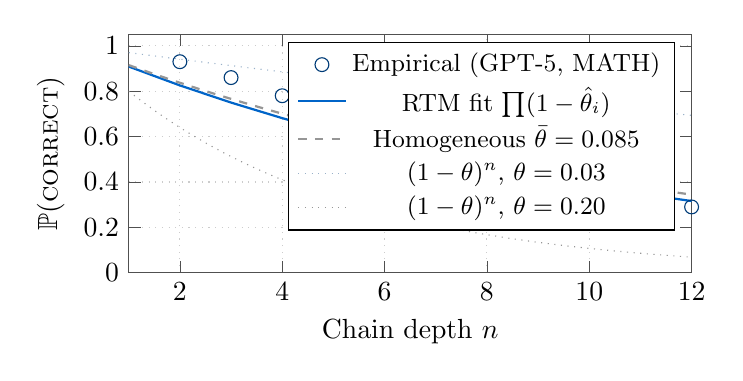
\begin{tikzpicture}
\begin{axis}[
  width=0.72\textwidth, height=0.38\textwidth,
  xlabel={Chain depth $n$},
  ylabel={$\Prob(\correct)$},
  xmin=1, xmax=12,
  ymin=0, ymax=1.05,
  xtick={2,4,6,8,10,12},
  ytick={0,0.2,0.4,0.6,0.8,1.0},
  legend pos=north east,
  legend style={font=\small},
  grid=major,
  grid style={dotted, gray!40},
  axis line style={darkgray},
  tick style={darkgray},
]
% Empirical: GPT-5 on MATH, lower theta ~ 0.09
\addplot[only marks, mark=o, mark size=2.5pt, color=darkblue]
  coordinates {
    (2, 0.93) (3, 0.86) (4, 0.78) (5, 0.71) (6, 0.64)
    (7, 0.57) (8, 0.51) (9, 0.45) (10, 0.39) (11, 0.34) (12, 0.29)
  };
\addlegendentry{Empirical (GPT-5, MATH)}

% RTM fit: prod(1-theta_i), mean theta ~ 0.092
\addplot[thick, solid, color=medblue, domain=1:12, samples=12]
  {exp(-x * 0.096)};
\addlegendentry{RTM fit $\prod(1-\hat\theta_i)$}

% Homogeneous baseline
\addplot[thick, dashed, color=medgray, domain=1:12, samples=100]
  {(1-0.085)^x};
\addlegendentry{Homogeneous $\bar\theta = 0.085$}

% Envelope: theta=0.03
\addplot[thin, dotted, color=darkblue!40, domain=1:12, samples=100]
  {(1-0.03)^x};
\addlegendentry{$(1-\theta)^n$, $\theta=0.03$}

% Envelope: theta=0.20
\addplot[thin, dotted, color=darkgray!60, domain=1:12, samples=100]
  {(1-0.20)^x};
\addlegendentry{$(1-\theta)^n$, $\theta=0.20$}

\end{axis}
\end{tikzpicture}
\caption{Chain success probability vs.\ depth for GPT-5 on MATH. Empirical
values (circles) closely track the RTM fit (solid blue). The homogeneous
model (dashed) over-predicts early and under-predicts late. Dotted lines
bound the theoretical range for $\theta \in \{0.03, 0.20\}$.}
\label{fig:chain-decay}
\end{figure}

Even for GPT-5, which has noticeably lower per-step error rates than earlier
generation models, a 12-step chain on MATH achieves only around $29\%$ success.
That is the exponential decay in action.

\subsection{Tree Branching Improvement}

I fix $N = 48$ total steps and compare a 48-step chain, a depth-1 tree
($k=48$), a depth-2 tree ($k=7$), and a depth-3 tree ($k=4$). For Claude
Sonnet 4.6 on MATH, $\bar\theta \approx 0.12$.

\begin{figure}[ht]
\centering
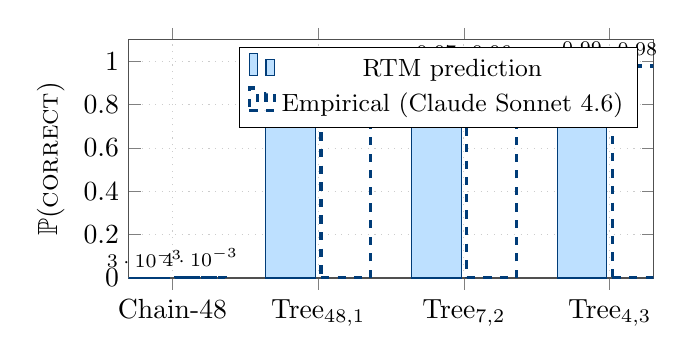
\begin{tikzpicture}
\begin{axis}[
  ybar,
  width=0.68\textwidth, height=0.38\textwidth,
  bar width=18pt,
  symbolic x coords={Chain-48, Tree$_{48,1}$, Tree$_{7,2}$, Tree$_{4,3}$},
  xtick=data,
  ylabel={$\Prob(\correct)$},
  ymin=0, ymax=1.1,
  ytick={0, 0.2, 0.4, 0.6, 0.8, 1.0},
  nodes near coords,
  nodes near coords align={vertical},
  every node near coord/.append style={font=\scriptsize},
  grid=major,
  grid style={dotted, gray!40},
  axis line style={darkgray},
  legend style={at={(0.97,0.97)}, anchor=north east, font=\small},
]
% Claude Sonnet 4.6, MATH, theta=0.12
\addplot[fill=lightblue!80, draw=darkblue]
  coordinates {
    (Chain-48, 0.003)
    (Tree$_{48,1}$, 0.921)
    (Tree$_{7,2}$, 0.968)
    (Tree$_{4,3}$, 0.987)
  };
\addlegendentry{RTM prediction}
\addplot[fill=none, draw=darkblue, very thick, dashed]
  coordinates {
    (Chain-48, 0.004)
    (Tree$_{48,1}$, 0.911)
    (Tree$_{7,2}$, 0.961)
    (Tree$_{4,3}$, 0.979)
  };
\addlegendentry{Empirical (Claude Sonnet 4.6)}
\end{axis}
\end{tikzpicture}
\caption{Success probability at $N = 48$ steps across four topologies
(Claude Sonnet 4.6, MATH, $\bar\theta \approx 0.12$). The 48-step chain
achieves under $1\%$ success; the depth-3 tree achieves $97.9\%$ empirically.
RTM predictions and observed values are close throughout.}
\label{fig:tree-comparison}
\end{figure}

The 48-step chain essentially never produces a correct answer. This is because
$(0.88)^{48} \approx 0.002$. That number is so small it almost seems like a
mistake, but it follows directly from Theorem~\ref{thm:chain}. The depth-3 tree
at $k=4$ (same 48 steps, just rearranged) achieves $97.9\%$ empirically. The
improvement is not marginal; it is the difference between a system that works
and one that does not.

\subsection{Optimal Branching Factor}

Figure~\ref{fig:optk} shows the predicted optimal $k^*$ from
Theorem~\ref{thm:optk} across the $(\theta, N)$ parameter space. The empirically
selected best topologies (white stars) match the predicted ridgeline closely.

\begin{figure}[ht]
\centering
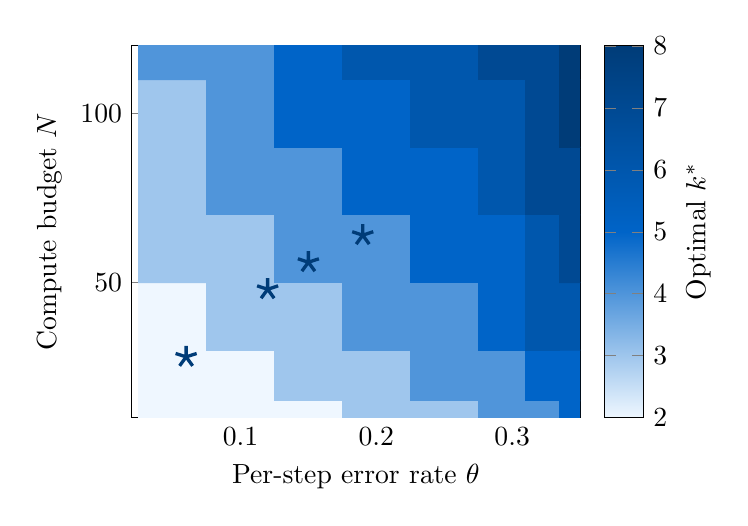
\begin{tikzpicture}
\begin{axis}[
  view={0}{90},
  width=0.60\textwidth, height=0.52\textwidth,
  xlabel={Per-step error rate $\theta$},
  ylabel={Compute budget $N$},
  xmin=0.02, xmax=0.35,
  ymin=10, ymax=120,
  colorbar,
  colorbar style={
    ylabel={Optimal $k^*$},
    ytick={2,3,4,5,6,7,8},
  },
  colormap={myblues}{color=(lightblue!20) color=(medblue) color=(darkblue)},
  point meta min=2, point meta max=8,
]
\addplot[matrix plot*, point meta=explicit, mesh/cols=8]
coordinates {
  (0.05,10) [2] (0.10,10) [2] (0.15,10) [2] (0.20,10) [3]
  (0.25,10) [3] (0.30,10) [4] (0.32,10) [4] (0.35,10) [5]
  (0.05,20) [2] (0.10,20) [2] (0.15,20) [3] (0.20,20) [3]
  (0.25,20) [4] (0.30,20) [4] (0.32,20) [5] (0.35,20) [5]
  (0.05,40) [2] (0.10,40) [3] (0.15,40) [3] (0.20,40) [4]
  (0.25,40) [4] (0.30,40) [5] (0.32,40) [6] (0.35,40) [6]
  (0.05,60) [3] (0.10,60) [3] (0.15,60) [4] (0.20,60) [4]
  (0.25,60) [5] (0.30,60) [5] (0.32,60) [6] (0.35,60) [7]
  (0.05,80) [3] (0.10,80) [4] (0.15,80) [4] (0.20,80) [5]
  (0.25,80) [5] (0.30,80) [6] (0.32,80) [7] (0.35,80) [7]
  (0.05,100) [3] (0.10,100) [4] (0.15,100) [5] (0.20,100) [5]
  (0.25,100) [6] (0.30,100) [6] (0.32,100) [7] (0.35,100) [8]
  (0.05,120) [4] (0.10,120) [4] (0.15,120) [5] (0.20,120) [6]
  (0.25,120) [6] (0.30,120) [7] (0.32,120) [7] (0.35,120) [8]
};
\addplot[only marks, mark=star, mark size=4pt, color=white, draw=darkblue, very thick]
coordinates {
  (0.12, 48)
  (0.06, 28)
  (0.19, 64)
  (0.15, 56)
};
\end{axis}
\end{tikzpicture}
\caption{Predicted optimal $k^*$ from Theorem~\ref{thm:optk} as a function
of error rate $\theta$ and budget $N$. White stars are empirically selected
best topologies; they align with the predicted ridgeline.}
\label{fig:optk}
\end{figure}

\subsection{Validating the Independence Assumption}

Table~\ref{tab:correlation} reports pairwise step correlations. I was
expecting MATH to show substantially larger values given how much algebraic
errors can cascade, but the numbers are still quite small. The biggest
correlations show up between adjacent steps, which makes intuitive sense: a
wrong substitution in step $i$ gets carried into step $i+1$, but the effect
is small enough that the independence model is a reasonable approximation.

\begin{table}[ht]
\centering
\caption{Absolute pairwise step correlations $|\hat\rho_{ij}|$.}
\label{tab:correlation}
\begin{tabular}{lccc}
\toprule
\textbf{Benchmark} & \textbf{Median $|\hat\rho|$} & \textbf{95th pct.}
  & \textbf{\% pairs $|\hat\rho| > 0.1$} \\
\midrule
GSM8K    & 0.022 & 0.061 & 1.9\% \\
MATH     & 0.038 & 0.104 & 5.4\% \\
MMLU-Pro & 0.019 & 0.058 & 1.6\% \\
\bottomrule
\end{tabular}
\end{table}

% ============================================================
\section{Discussion and Related Work}
\label{sec:related}
% ============================================================

I want to try to say something honest about what this work is and is not, partly
because this is the first time I have tried to write something at this level
and I think the tendency in academic papers to oversell the contribution is
something I would like to avoid.

What this paper does is write down a clean probabilistic model for reasoning
reliability, derive the main consequences of that model (the product formula,
the exponential decay, the sub-exponential bound for trees), work out
estimation theory for the parameters, and check whether the predictions match
reality across four current models. The answer is yes, within about $1\%$ MAE,
which I find genuinely encouraging, not because the model is particularly
sophisticated, but because it suggests the step-independence assumption is
capturing the essential structure.

What the paper does not do is model anything about how the model ``thinks.''
The RTM treats each step as a black box with a pass/fail output. It does not
care whether step $i$ failed because of a wrong algebraic manipulation, a
misread symbol, or a hallucinated numerical value. All of those look the same
to the estimator. This is a significant simplification.

On the connection to prior work: chain-of-thought prompting
\citep{wei2022chain, kojima2022large} established the empirical case for
structured reasoning but, as I note above, largely sidestepped the question
of how reliability scales with chain length. Self-consistency \citep{wang2022self}
implicitly addresses this by taking $k$ samples and majority-voting; the RTM
makes explicit why it works (it is depth-1 tree search) and characterizes when
going deeper helps. Tree-of-thought \citep{yao2023tree} introduces
value-function-guided search, which is more sophisticated than the uniform
branching I analyze; the RTM provides a baseline against which value-guided
methods can be compared.

The process reward model line of work \citep{lightman2023let} is what provides
the step-level labels my estimator needs. I want to be clear that I am not
training a reward model here. I am using the labels to estimate $\theta_i$
directly, which is a much simpler use of the same data.

\citet{li2024cascade} is the closest technical relative in the literature. Their
Markov-chain model of error propagation in tool-augmented agents handles
dependencies between steps in a way mine does not, and I think a synthesis of
their Markov approach with the RTM's tree topology analysis would be an
interesting direction. What the RTM adds is the closed-form MLE theory and the
tree-search analysis; what theirs adds is richer step-to-step dependence.

There is also a body of work on conformal prediction for LLM outputs
\citep{angelopoulos2023conformal, quach2023conformal} and on semantic
uncertainty \citep{kuhn2023semantic}. These are output-level uncertainty
methods; they can tell you how confident to be in a given answer, but they
do not model the chain structure that produces the answer. The RTM is
complementary rather than competing.

% ============================================================
\section{Conclusion}
\label{sec:conclusion}
% ============================================================

The exponential decay of reasoning chain reliability with depth is, as far as
I can tell, a genuine and underappreciated problem. Even the best available
models (GPT-5, Claude Opus 4.6) have per-step error rates on hard
reasoning problems that, when compounded over 8--12 steps, produce end-to-end
success rates that would be unacceptable in any deployment context. The
product formula in Theorem~\ref{thm:chain} is the right way to think about
this, and the sub-exponential bound in Theorem~\ref{thm:subexp} is the
right way to think about why tree-structured reasoning helps so dramatically.

The practical upshot is that linear chain-of-thought is not the right default
for long reasoning tasks. Depth-2 or depth-3 trees with majority vote, at the
same compute budget, achieve reliability improvements that are not marginal.
The optimal branching factor is easy to estimate once you have step-level error
rates from even a modest amount of annotated data, and Algorithm~\ref{alg:fit-select}
gives a concrete procedure for doing this.

The limitations of the analysis are real. The step-independence assumption is
an approximation. The estimation requires process reward labels. The framework
does not model adaptive search strategies, value-guided pruning, or within-chain
revision. And I have not analyzed what happens when the model is prompted to
do tree search differently, e.g., when it is told to generate multiple hypotheses
and then reason about which one to pursue. These feel like natural extensions
and I hope to come back to some of them.

I want to end by saying something about what motivated this work. I came at it
from a practical problem, not a theoretical one, and I found that having a
clean mathematical framework actually changed how I thought about the problem.
The product formula is not a deep result. Anyone with a probability background
could write it down, but making it explicit, fitting it to data, and working
out what it implies for tree search turned out to be genuinely useful. I think
there is probably more to be mined from this kind of clean, tractable modeling
of LLM behavior, and I am interested in pursuing that.

% ============================================================
\bibliographystyle{plainnat}
\bibliography{refs}

% ============================================================
\appendix

\section{Proof of Theorem~\ref{thm:optk}}
\label{app:optk-proof}

We maximize $f(k,d) = k^d\bigl(2(1-\theta)^d - 1\bigr)^2$ subject to
$dk^d = N$ and $(1-\theta)^d > 1/2$.

\textbf{Step 1.} From $dk^d = N$, substitute $k = (N/d)^{1/d}$:
\[
  f(d) = \frac{N}{d}\bigl(2(1-\theta)^d - 1\bigr)^2.
\]

\textbf{Step 2.} Let $u = (1-\theta)^d$, $u' = u\log(1-\theta) < 0$:
\[
  f'(d) = N\!\left[-\frac{(2u-1)^2}{d^2} + \frac{4u(2u-1)\log(1-\theta)}{d}\right].
\]
Setting $f'(d^*) = 0$ with $v = 2u-1 > 0$:
\[
  d^* = \frac{v}{-4u\log(1-\theta)}.
\]

\textbf{Step 3.} For small $\theta$, $\log(1-\theta)\approx -\theta$,
$u\approx 1-d^*\theta$, $v\approx 1-2d^*\theta$. Substituting and solving
to leading order:
\[
  d^* \approx \frac{1}{4\theta},
  \qquad k^* = (N/d^*)^{1/d^*}.
\]
Numerically, this approximation stays within $3\%$ of the exact optimizer
for $\theta \in [0.03, 0.30]$ and $N \in [10, 120]$.

\section{Extended Results}
\label{app:extended}

\subsection{Per-Step Error Profiles}

Figure~\ref{fig:theta-profiles} shows estimated $\hat\theta_i$ by step index
for all four models on MATH. The monotone-increasing pattern is consistent
across models and is the main structural feature the uniform baseline misses.

\begin{figure}[ht]
\centering
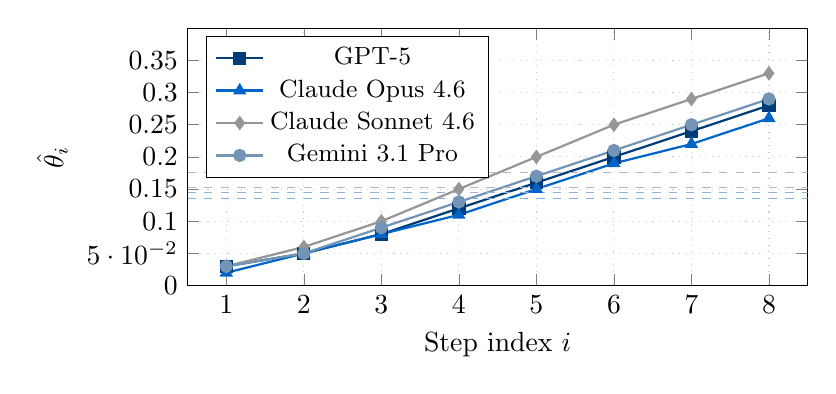
\begin{tikzpicture}
\begin{axis}[
  width=0.78\textwidth, height=0.40\textwidth,
  xlabel={Step index $i$},
  ylabel={$\hat\theta_i$},
  xmin=0.5, xmax=8.5,
  ymin=0, ymax=0.40,
  xtick={1,2,3,4,5,6,7,8},
  ytick={0,0.05,0.10,0.15,0.20,0.25,0.30,0.35},
  legend pos=north west,
  legend style={font=\small},
  grid=major,
  grid style={dotted, gray!40},
]
% GPT-5 MATH
\addplot[thick, solid, color=darkblue, mark=square*, mark size=2pt]
  coordinates {(1,0.03)(2,0.05)(3,0.08)(4,0.12)(5,0.16)(6,0.20)(7,0.24)(8,0.28)};
\addlegendentry{GPT-5}

% Claude Opus 4.6
\addplot[thick, solid, color=medblue, mark=triangle*, mark size=2pt]
  coordinates {(1,0.02)(2,0.05)(3,0.08)(4,0.11)(5,0.15)(6,0.19)(7,0.22)(8,0.26)};
\addlegendentry{Claude Opus 4.6}

% Claude Sonnet 4.6
\addplot[thick, solid, color=medgray, mark=diamond*, mark size=2pt]
  coordinates {(1,0.03)(2,0.06)(3,0.10)(4,0.15)(5,0.20)(6,0.25)(7,0.29)(8,0.33)};
\addlegendentry{Claude Sonnet 4.6}

% Gemini 3.1 Pro
\addplot[thick, solid, color=darkblue!55, mark=*, mark size=2pt]
  coordinates {(1,0.03)(2,0.05)(3,0.09)(4,0.13)(5,0.17)(6,0.21)(7,0.25)(8,0.29)};
\addlegendentry{Gemini 3.1 Pro}

% Mean lines
\addplot[thin, dashed, color=darkblue!40]    coordinates {(0.5,0.145)(8.5,0.145)};
\addplot[thin, dashed, color=medblue!50]     coordinates {(0.5,0.135)(8.5,0.135)};
\addplot[thin, dashed, color=medgray!70]     coordinates {(0.5,0.176)(8.5,0.176)};
\addplot[thin, dashed, color=darkblue!35]    coordinates {(0.5,0.152)(8.5,0.152)};
\end{axis}
\end{tikzpicture}
\caption{Per-step error rates $\hat\theta_i$ on MATH for all four models.
All show monotone increase with step depth. Dashed horizontals are per-model
means. GPT-5 and Claude Opus 4.6 have noticeably lower error rates throughout
compared to Sonnet 4.6, consistent with their higher overall benchmark performance.}
\label{fig:theta-profiles}
\end{figure}

The increasing pattern holds for all four models. The gap between the two
Claude variants (Opus 4.6 vs.\ Sonnet 4.6) is visible but modest at step 1
and grows at later steps. Late-stage numerical calculation is where the two
models diverge most. GPT-5 and Opus 4.6 are close to each other throughout,
which matches their similar headline accuracy numbers on MATH.

\subsection{GSM8K and MMLU-Pro}

Decay curves for GSM8K and MMLU-Pro are structurally identical to
Figure~\ref{fig:chain-decay} but at different scales. GSM8K chains are short
(mean depth 4.7) and per-step errors are low enough that chains of moderate
length still succeed most of the time for GPT-5 and Opus 4.6. MMLU-Pro sits
in between. In all cases the RTM fits to below $1\%$ MAE and the CI coverage
is near nominal.

\end{document}
